\section{Applications du modèle}

\begin{frame}
    \frametitle{Applications}
    \framesubtitle{Plan}
    \textbf{Deux applications du programme}\\
    \begin{itemize}
        \item <2-> Evaluation du trafic maximal d'un quai de métro
        \item <3-> Vérification de résultats scientifiques connus
    \end{itemize}
\end{frame}


\begin{frame}
    \frametitle{Evaluation du trafic maximal}
    \framesubtitle{Cadre des tests}
    \textbf{Cadre} : quai de métro à l'arrivée d'un train \\[.3cm]
    \begin{figure}
        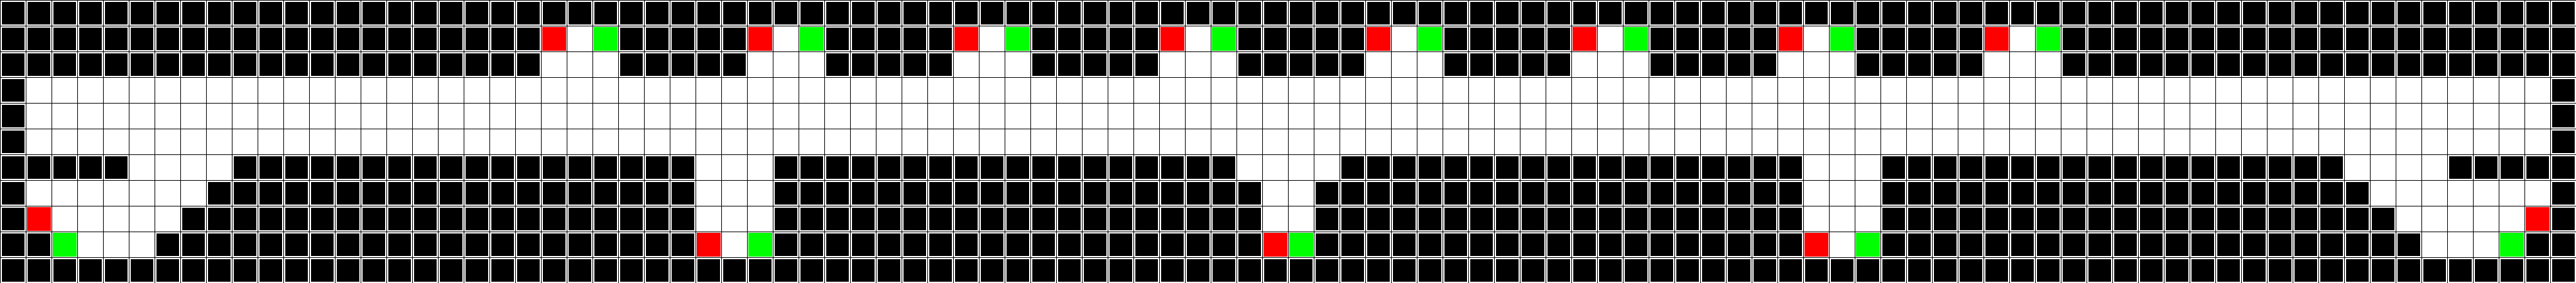
\includegraphics[width=1\textwidth]{figures/Fig05}
    \end{figure}
    \begin{columns}
        \begin{column}{0.35\textwidth}
            \tiny{\fcolorbox{black}{black}{\rule{0pt}{6pt}\rule{6pt}{0pt}}\quad Mur (case infranchissable) \\
                \fcolorbox{black}{white}{\rule{0pt}{6pt}\rule{6pt}{0pt}}\quad Quai (case franchissable) \\
                \fcolorbox{black}{green}{\rule{0pt}{6pt}\rule{6pt}{0pt}}\quad Sortie \\
                \fcolorbox{black}{red}{\rule{0pt}{6pt}\rule{6pt}{0pt}}\quad Entrée \\}
        \end{column}
        \begin{column}{0.7\textwidth}
            \onslide<2-> Longueur du quai : \num{100} \si{\metre} \\
            \onslide<3-> Largeur du quai : \num{3} \si{\metre}  \\
            \bigskip
            \onslide<4-> Surface de la partie centrale : $50 \times 3 = 150$ \si{\metre \squared}   \\[.5cm]
            \onslide<5-> Ainsi, le quai est dimensionné pour recevoir
            \begin{itemize}
                \item <6-> dans un cas normal : $150 \times 3 = 450$ usagers
                \item <7-> dans un cas critique : $150 \times 6 = 900$ usagers
            \end{itemize}
        \end{column}
    \end{columns}
\end{frame}


\begin{frame}
    \frametitle{Evaluation du trafic maximal}
    \framesubtitle{Protocole de test}
    \textbf{Protocole de test}
    \begin{itemize}
        \item <2-> relève du nombre d'étapes de simulation pour une population initiale donnée
        \item <3-> moyenne sur 20 mesures pour chaque point
        \item <4-> relève du nombre de simulations qui n'ont pas terminé pour chaque population initiale
    \end{itemize}
\end{frame}


\begin{frame}
    \frametitle{Evaluation du trafic maximal}
    \framesubtitle{Variation de la population initiale}
    \begin{tikzpicture}
        \begin{axis}[width=1\textwidth,height=.8\textheight,xlabel=Population initiale,ylabel=Etapes, legend style={at={(0.45,0.05)},anchor=south west},]
            \addplot table [y=temps, x=population]{data/pop_etapes_heuristique.txt};
            \addplot [red, mark = x, nodes near coords=2,every node near coord/.style={anchor=-90}] coordinates {( 1000, 148)};
            \addplot [red, mark = x, nodes near coords=5,every node near coord/.style={anchor=-90}] coordinates {( 1050, 151)};
            \addplot [red, mark = x, nodes near coords=1,every node near coord/.style={anchor=-90}] coordinates {( 950, 146)};
            \addplot [red, mark = x, nodes near coords=10,every node near coord/.style={anchor=+90}] coordinates {( 1100, 150)};
            \addplot [red, mark = x, nodes near coords=13,every node near coord/.style={anchor=-90}] coordinates {( 1150, 161)};
            \addplot [red, mark = x, nodes near coords=19,every node near coord/.style={anchor=+90}] coordinates {( 1200, 173)};
            \addplot [red, mark = x, nodes near coords=20,every node near coord/.style={anchor=+90}] coordinates {( 1250, 501)};
            \addplot [red, mark = x, nodes near coords=20,every node near coord/.style={anchor=-90}] coordinates {( 1300, 501)};
            \addplot [red, mark = x, nodes near coords=20,every node near coord/.style={anchor=+90}] coordinates {( 1350, 501)};
            \draw[dashed][black] (-100, 501) -- node[below] {limite fixée} (1600, 501);
            \legend{itérations par pop. initiale, simulations qui se figent};
        \end{axis}
        \node[align=center,font=\bfseries, yshift=1em] (title)
        at (current bounding box.north)
        {Durée de simulation pour une population initiale donnée};
    \end{tikzpicture}
\end{frame}


\begin{frame}
    \frametitle{Evaluation du trafic maximal}
    \framesubtitle{Conclusion}
    \begin{tikzpicture}
        \begin{axis}[width=1\textwidth,width=1\textwidth, height=.4\textheight,xlabel=Population initiale,legend style={at={(0.45,0.05)},anchor=south west},]
            \addplot table [y=temps, x=population]{data/pop_etapes_heuristique.txt};
            \addplot [red, mark = x, nodes near coords=1,every node near coord/.style={anchor=-90}] coordinates {( 950, 146)};
            \addplot [red, mark = x, nodes near coords=2,every node near coord/.style={anchor=-90}] coordinates {( 1000, 148)};
            \addplot [red, mark = x, nodes near coords=5,every node near coord/.style={anchor=-90}] coordinates {( 1050, 151)};
            \addplot [red, mark = x, nodes near coords=10,every node near coord/.style={anchor=+90}] coordinates {( 1100, 150)};
            \addplot [red, mark = x, nodes near coords=13,every node near coord/.style={anchor=-90}] coordinates {( 1150, 161)};
            \addplot [red, mark = x, nodes near coords=19,every node near coord/.style={anchor=+90}] coordinates {( 1200, 173)};
            \addplot [red, mark = x, nodes near coords=20,every node near coord/.style={anchor=+90}] coordinates {( 1250, 501)};
            \addplot [red, mark = x, nodes near coords=20,every node near coord/.style={anchor=-90}] coordinates {( 1300, 501)};
            \addplot [red, mark = x, nodes near coords=20,every node near coord/.style={anchor=+90}] coordinates {( 1350, 501)};
            \draw[dashed][black] (-100, 501) -- node[below] {limite fixée} (1600, 501);
        \end{axis}
        \node[align=center,font=\bfseries, yshift=1em] (title)
        at (current bounding box.north)
        {Durée de simulation pour une population initiale donnée};
    \end{tikzpicture}
    \onslide<2-> On retrouve bien des blocages à partir d'une population initiale d'environ 950 personnes. \\[.5cm]
    \onslide<3-> Le modèle renvoie bien un résultat cohérent avec la valeur estimée.
\end{frame}


\begin{frame}
    \frametitle{Divsion du flux}
    \framesubtitle{Présentation du phénomène}
    \textbf{Placement d'un obstacle devant une sortie} \\
    Ce phénomène s'interprète comme une division du flux incident
    \begin{columns}
        \begin{column}{0.475\textwidth}
            \begin{figure}
                Illustration
                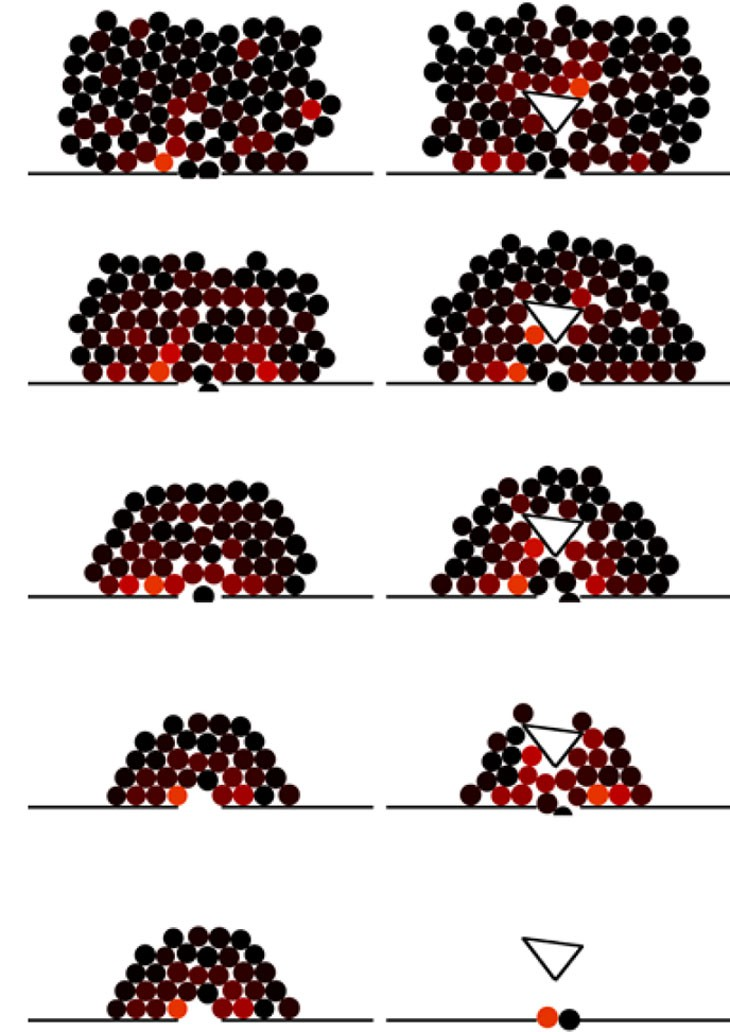
\includegraphics[height=.58\textheight]{figures/Fig07}
                \imagesource{\href{https://www.pourlascience.fr/sd/mathematiques/la-foule-en-equations-17252.php}{Pour La Science N°501}}
            \end{figure}
        \end{column}
        \only<2>{\begin{column}{0.475\textwidth}
                \begin{figure}
                    On souhaite mettre en valeur ce phénomène : \\[.2cm]
                    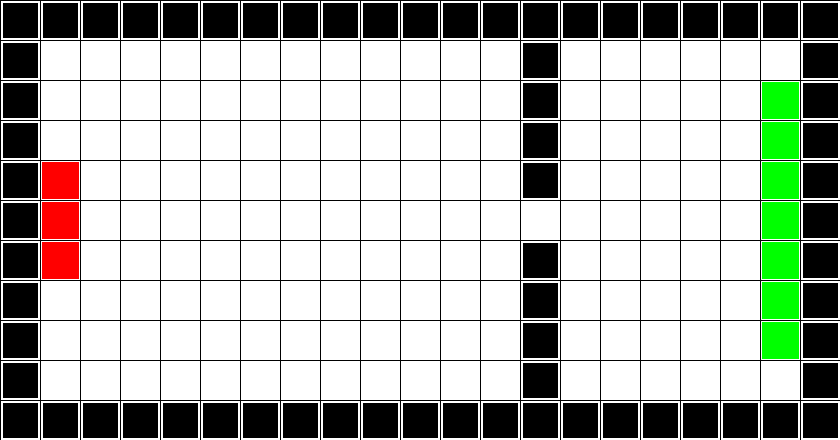
\includegraphics[width=.6 \textwidth]{figures/Fig09} \\[.3cm]
                    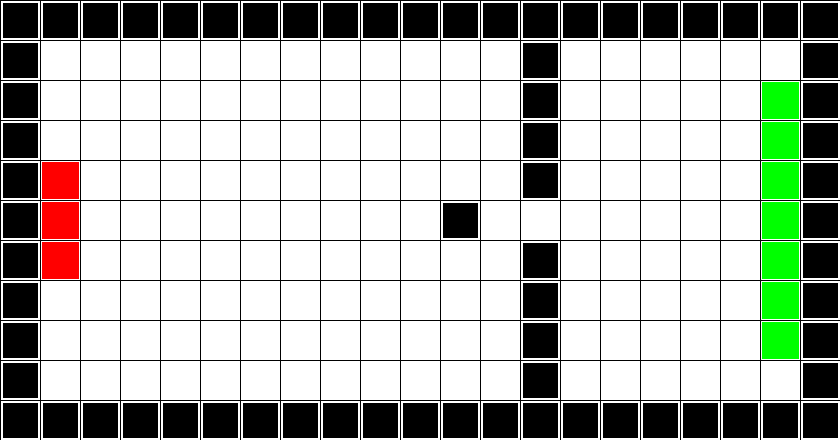
\includegraphics[width=.6\textwidth]{figures/Fig08}
                \end{figure}
            \end{column}
        }
    \end{columns}
\end{frame}


\begin{frame}
    \frametitle{Division du flux}
    \framesubtitle{Protocole de test}
    \textbf{Protocole de test}
    \begin{itemize}
        \item <2-> relève du nombre d'étapes de simulation pour une population initiale donnée
        \item <3-> relève du nombre de cases pour lesquelles la densité a dépassé 5 personnes/m²
        \item <4-> moyenne sur 50 mesures pour chaque point
    \end{itemize}
\end{frame}


\begin{frame}
    \frametitle{Division du flux}
    \framesubtitle{Résultats du programme}
    \begin{tikzpicture}
        \begin{axis}[width=1\textwidth,height=.8\textheight,xlabel=Population,ylabel=étapes\ \ \ , legend style={at={(0.05,0.95)},anchor=north west},]
            \addplot table [blue, y=temps, x=population]{data/pop_sans_obstacle.txt};
            \addplot table [red, y=temps, x=population]{data/pop_avec_obstacle.txt};
            \only<2->{\addplot table [blue, y=dens, x=population]{data/pop_sans_obstacle.txt};
                \addplot table [red, y= dens, x=population]{data/pop_avec_obstacle.txt};}
            \tiny{\legend{durée sans obstacle, durée avec obstacle, occurences de densités $\geq 5$ p/m² sans obstacle, occurences de densités $\geq 5$ p/m² avec obstacle}};
        \end{axis}
        \node[align=center,font=\bfseries, yshift=1em] (title)
        at (current bounding box.north)
        {Durée de simulation pour une population initiale donnée};
    \end{tikzpicture}
\end{frame}


\begin{frame}
    \frametitle{Division du flux}
    \framesubtitle{Conclusion}
    \begin{tikzpicture}
        \begin{axis}[width=1\textwidth,height=.4\textheight,xlabel=Population,legend style={at={(0.05,0.95)},anchor=north west},]
            \addplot table [blue, y=temps, x=population]{data/pop_sans_obstacle.txt};
            \addplot table [red, y=temps, x=population]{data/pop_avec_obstacle.txt};
            \addplot table [blue, y=dens, x=population]{data/pop_sans_obstacle.txt};
            \addplot table [red, y= dens, x=population]{data/pop_avec_obstacle.txt};
        \end{axis}
        \node[align=center,font=\bfseries, yshift=1em] (title)
        at (current bounding box.north)
        {Durée de simulation pour une population initiale donnée};
    \end{tikzpicture}
    On constate une évacuation plus rapide avec l'obstacle ainsi qu'un nombre moins important de situations dangereuses pour les agents. \\[1cm]
    Le modèle renvoie bien un résultat en accord avec le phénomène décrit.
\end{frame}


\begin{frame}
    \frametitle{Conclusion}
    La modélisation informatique de foules a de nombreuses applications :\\
    \begin{itemize}
        \item <2-> Sécurité et dimensionnement des infrastructures
        \item <3-> Etude de comportement sociaux
        \item <4-> Cinéma, jeux vidéo
    \end{itemize}
    \bigskip
    \bigskip
    \huge{Merci de votre attention.}
\end{frame}